\documentclass[11pt]{article}
\usepackage{graphicx}
\usepackage{booktabs}
\usepackage{amsmath}
\usepackage{geometry}
\geometry{margin=1in}

\title{Budgeted Repeated Second-Price Auction: Stage Game, Dynamics, and Evidence}
\author{PS-1 Report Scaffold}
\date{\today}

\begin{document}
\maketitle

\section{Introduction}
We study a modified repeated second-price auction with per-round budgets and refills.
This scaffold includes placeholders for figures, tables, and references.

\section{Model}
Two players, private values $v_i^t \sim \mathcal{U}[60,100]$, initial budgets $B_i^0>100$, per-round refill $r\in(0,60)$. Bids are capped by budgets, second-price rule, budgets update with refill and payments.

\section{Stage Game}
We discretize bids at step $\Delta_b$ and compute Nash equilibria using NashPy.
Figure~\ref{fig:stage} shows heatmaps (to be inserted).

\section{Dynamic Program}
Finite-horizon backward induction over a budget grid for a threshold policy class $b=\min\{v,\tau(B),B\}$; opponent truth-tells.

\section{Simulation Results}
Figure~\ref{fig:pricepath} shows mean price vs. round with 95\% CI.
\begin{figure}[h]
  \centering
  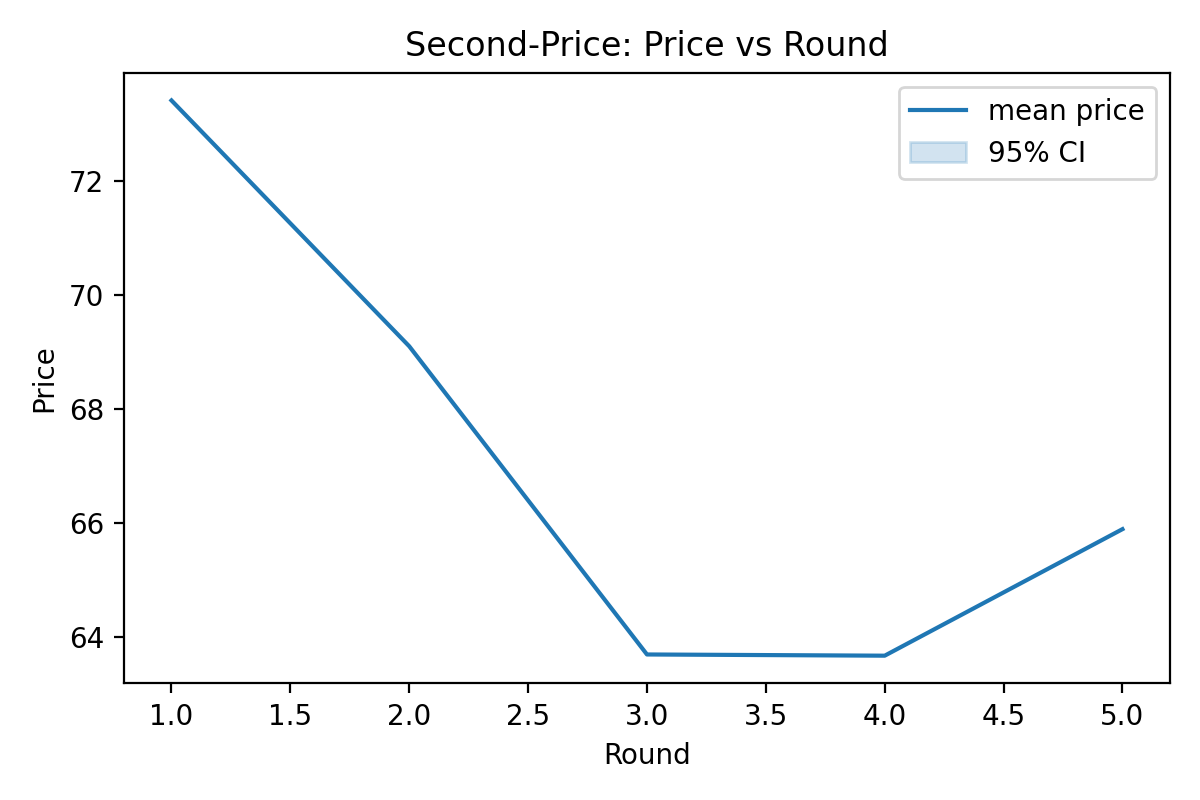
\includegraphics[width=0.7\linewidth]{figures/price_vs_round.png}
  \caption{Price vs. round under default parameters.}
  \label{fig:pricepath}
\end{figure}

\section{oTree Comparison}
We ingest oTree CSV and compare price paths and efficiency.

\section{Conclusion}
Summary of findings and future work.

% Bibliography stub
% \bibliographystyle{plain}
% \bibliography{refs}

\end{document}

